\documentclass{article}
\usepackage{enumitem}
\usepackage[utf8]{inputenc}
\usepackage{amsmath}
\usepackage{mathtools}
\usepackage{hyperref}
\usepackage{graphicx}
\usepackage{pdfpages}
\DeclarePairedDelimiter{\floor}{\lfloor}{\rfloor}
\title{Assignment 1}
\author{Mytraya Gattu, 180050032}
\date{14 August 2020}

\begin{document}

\maketitle

\section{Problem 1}
In what follows, $r$ is the radius of the hemispherical caps,$l$ the length and $m$ of the cell. It is given that, 
$$r=0.5\mu \text{m}$$
$$l=2\mu \text{m}$$
\begin{enumerate}[label=(\alph*)]
  \item Volume is given by $$V=\pi r^2 l + \frac{4}{3}\pi r^{3} = 2.094 \mu \text{m}^{3}$$
  Typical cell volume is $0.6-0.7 \mu \text{m}^{3}$
  \newline
  \url{https://en.wikipedia.org/wiki/Escherichia_coli}
  \item $m$ is the sum of the mass of water contained and that of the other substances. Since, density of water is $$10^3 \frac{\text{kg}}{\text{m}^3}=10^{-6} \frac{\text{pg}}{\mu \text{m}^3}$$
  We have
  $$m=10^{-6} \cdot \left(\frac{2}{3} + 1.3\cdot \frac{1}{3}\right)\cdot V \text{pg} = 2.304 \cdot 10^{-3} \text{pg}$$
  
  Typical cell weight is $1\cdot 10^{-3} \text{pg}$ \newline \url{https://ecmdb.ca/e_coli_stats)}
\end{enumerate}
It is evident from the above calculations, that the it is the assumed shape of \textit{E. coli} which deviates greatly from what is true. 
\section{Problem 2}
    Let at the end of $9^{\text{th}}$ cycle there be $N$ nuclei at the surface. At the end of $13^{\text{th}}$ cycle, therefore there are $16N$ nuclei, which is given as $\approx 6000$. Hence, $$N \approx 375$$
    Since, every embryo must start from a single fertilized nucleus, at the end of $9^{\text{th}}$ cycle, there must be $2^{9} = 512$ nuclei in total. Therefore, the fraction of nuclei which migrated to the surface is$$\frac{375}{512} \approx 0.7324$$
    Following the notation of Problem 1, surface area of the spherocylinder is $$A=4\pi r^{2} + 2\pi r l = 4.3982\cdot 10^{-7} \text{m}^{2}$$ 
    Therefore, the areal density is $$1.3642\cdot10^{10} \frac{\text{nuclei}}{\text{m}^2}$$
    To find the length of the green region, I used the co-ordinate tool in Mathematica. \newline
	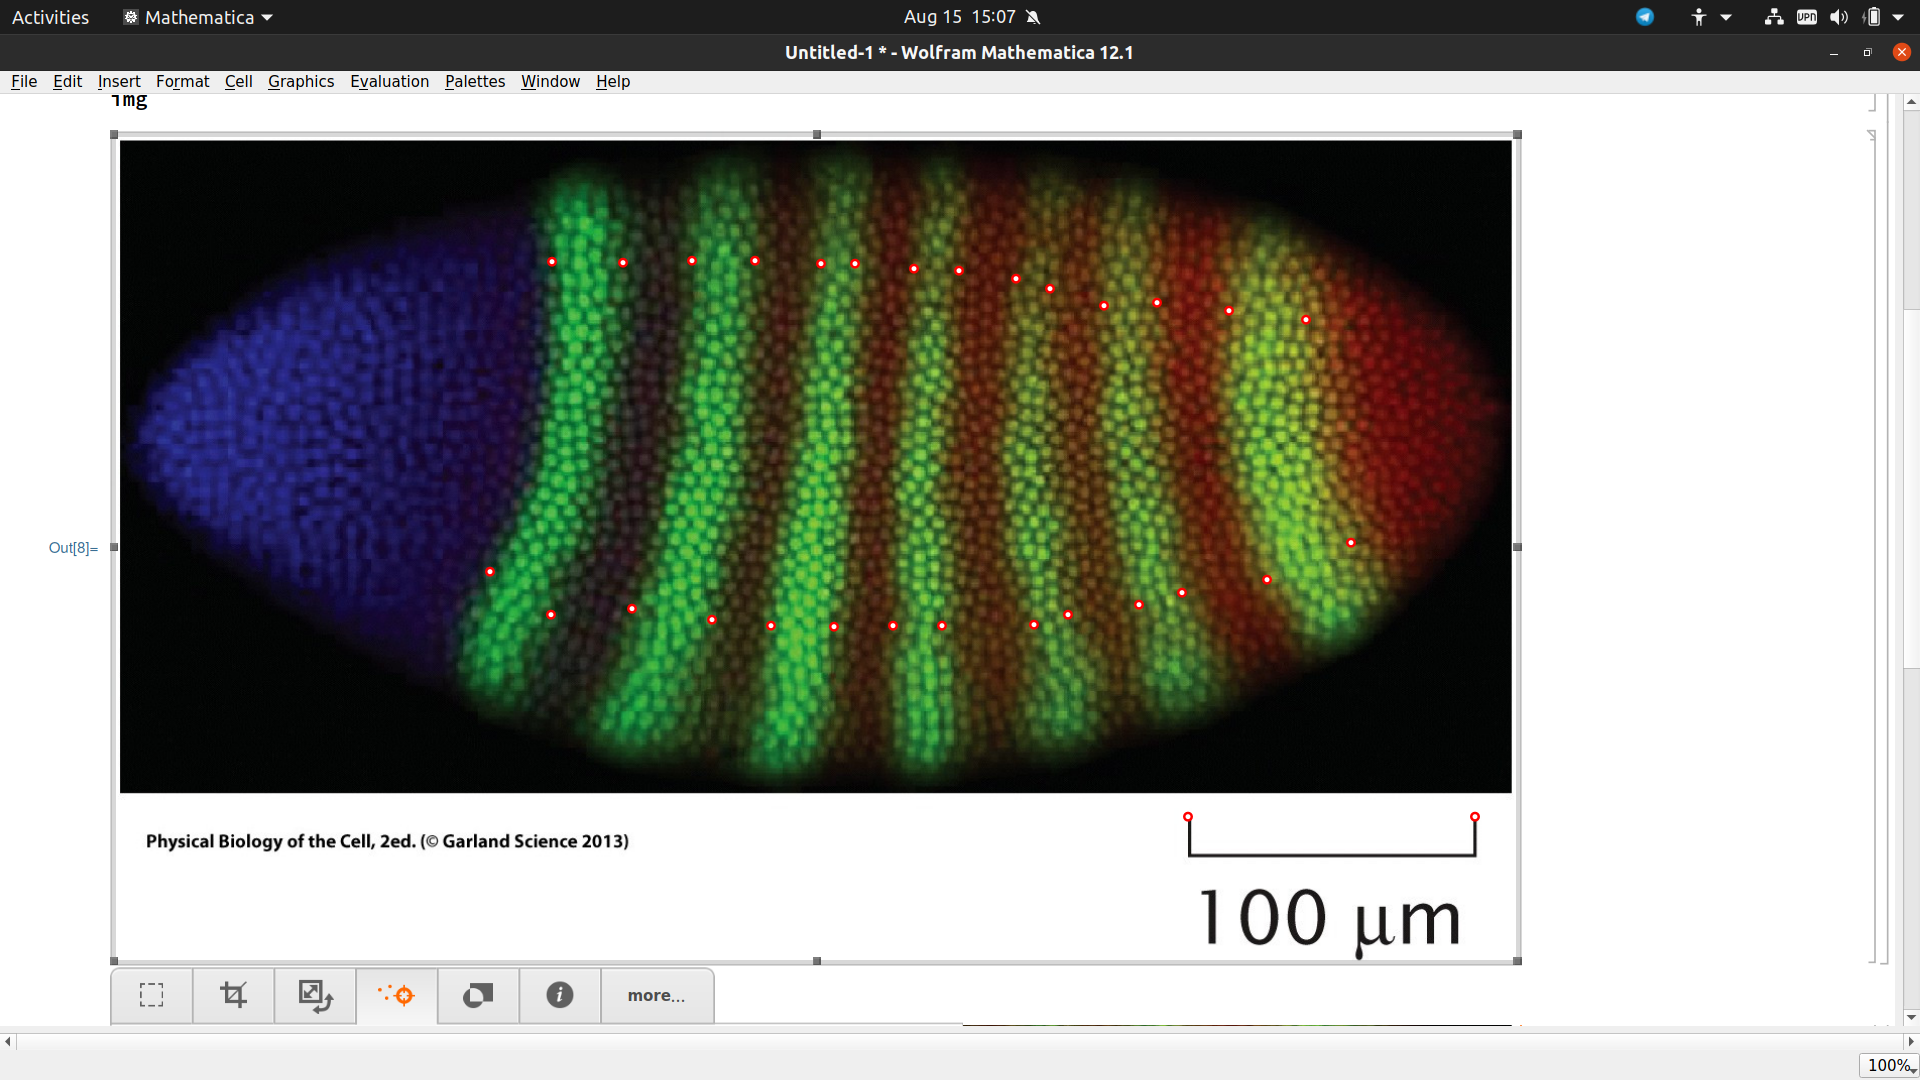
\includegraphics[width=10cm,height=10cm]{Screenshot from 2020-08-15 15-07-25.png} \newline
	Length of green region is
	$\approx 20.36 \mu \text{m}$. 
	Area is calculated, by isolating the green regions and finding the ratio between the number of pixels contained in these regions and the rest of the image. \newline
	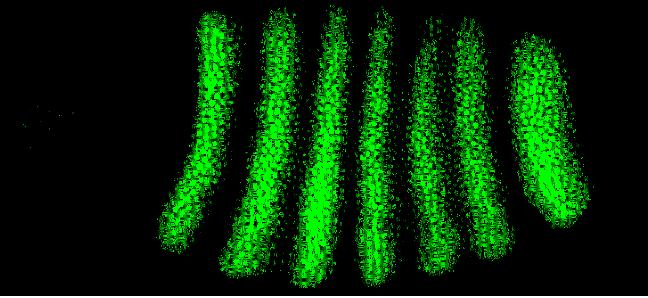
\includegraphics{bio.jpeg}
	\newline
	Using the areal density, number of cells in the green region(Even-skipped) is $\approx 198$.
	Similarly,number of cells in the red region(Caudal) is $\approx 139$ and number of cells in the blue region(Bicoid) is $\approx 58$. (Counting as a single surface)

\section{Problem 3}
\subsection{E. coli}
Mean of sequence length: $1892.0014318442154$ \newline
Standard deviation of sequence length: $3872.730811954928$ \newline
Mean of molecular mass: $289.0322422680412$ \newline
Standard deviation of molecular mass: $775.7631092745543$ \newline


\setlength{\voffset}{0cm}
\setlength{\hoffset}{0cm}

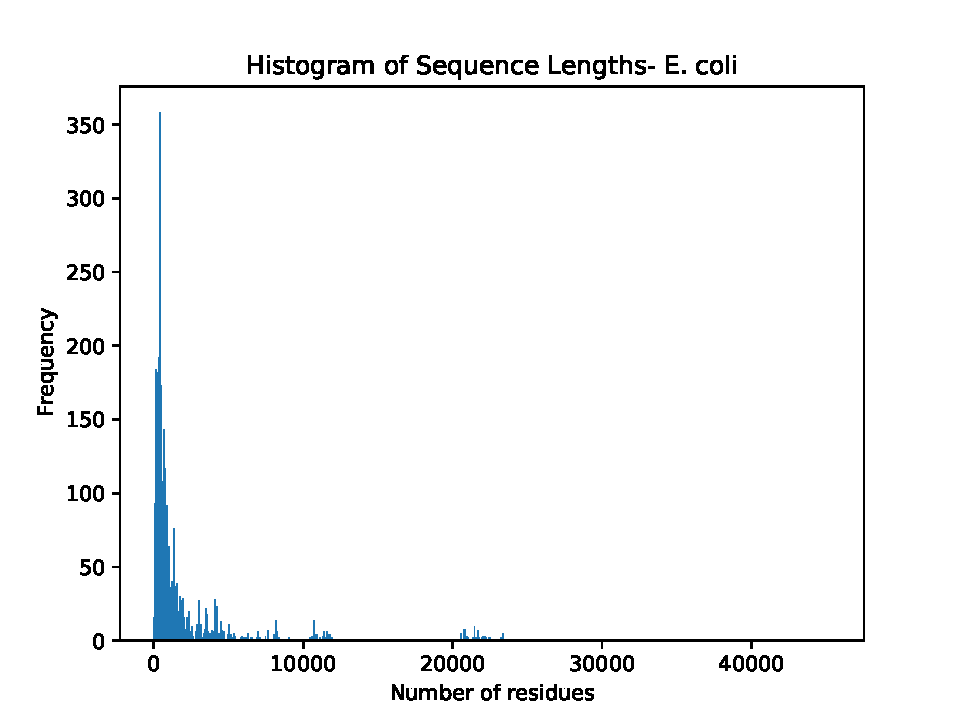
\includepdf[pages=-]{ecoli_length.pdf}

\setlength{\voffset}{-2.54cm}
\setlength{\hoffset}{-2.54cm}
\setlength{\voffset}{0cm}
\setlength{\hoffset}{0cm}

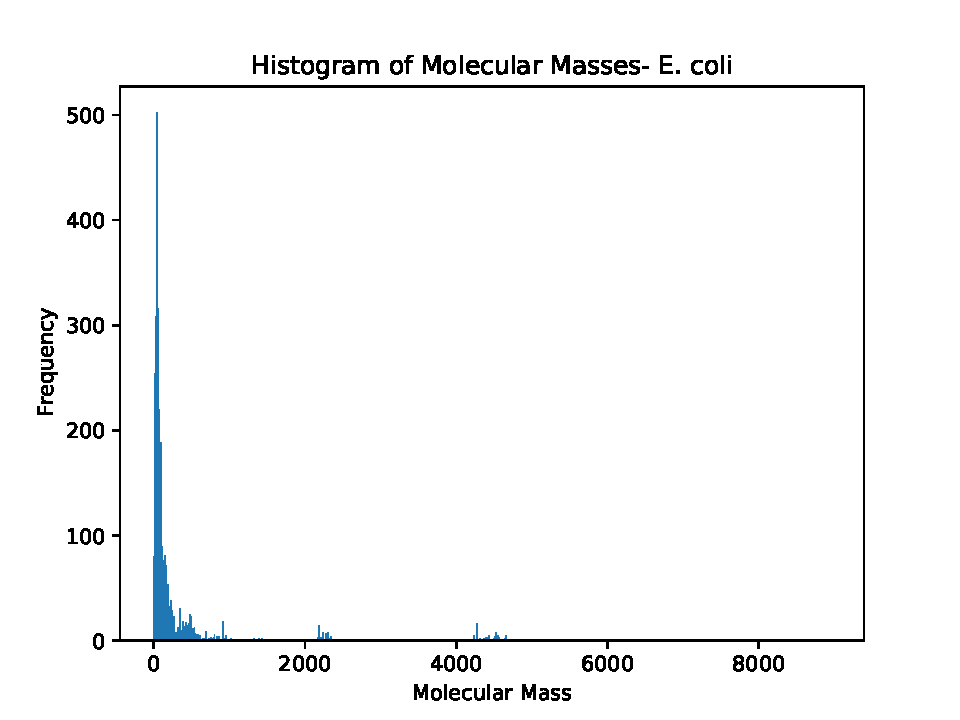
\includepdf[pages=-]{ecoli_mass.pdf}

\setlength{\voffset}{-2.54cm}
\setlength{\hoffset}{-2.54cm}
% \includepdf{}
\subsection{S. cerevisiae}
Mean of sequence length: $1287.8953846153847$ \newline
Standard deviation of sequence length: $2444.4862593462344$ \newline
Mean of molecular mass: $154.77802307692306$ \newline
Standard deviation of molecular mass: $313.30732277898954$ \newline

\setlength{\voffset}{0cm}
\setlength{\hoffset}{0cm}

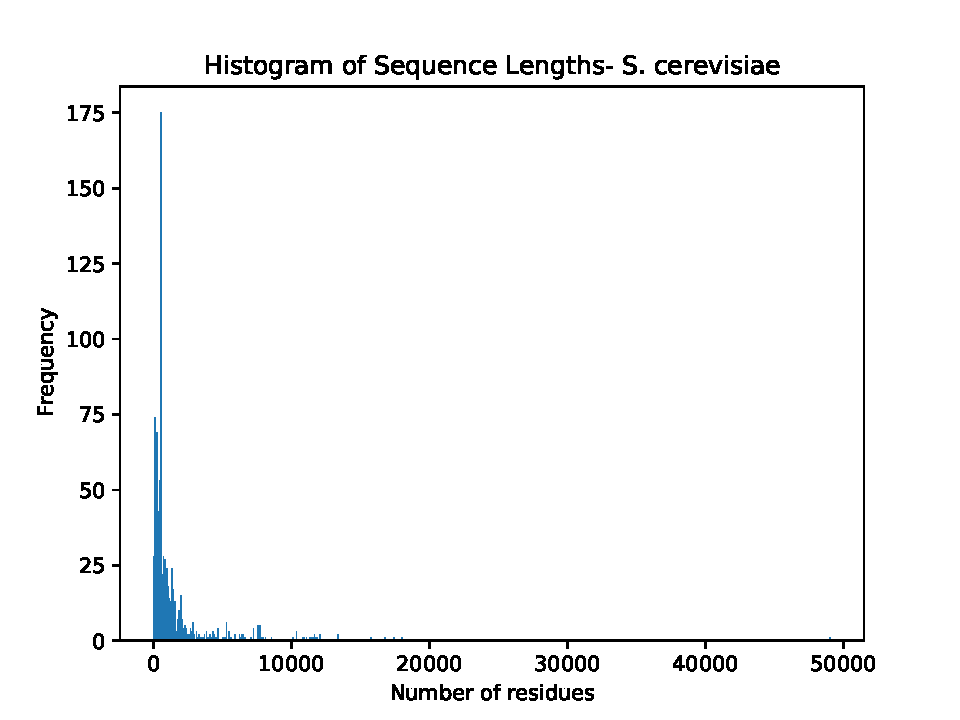
\includepdf[pages=-]{scerevisiae_length.pdf}

\setlength{\voffset}{-2.54cm}
\setlength{\hoffset}{-2.54cm}
\setlength{\voffset}{0cm}
\setlength{\hoffset}{0cm}

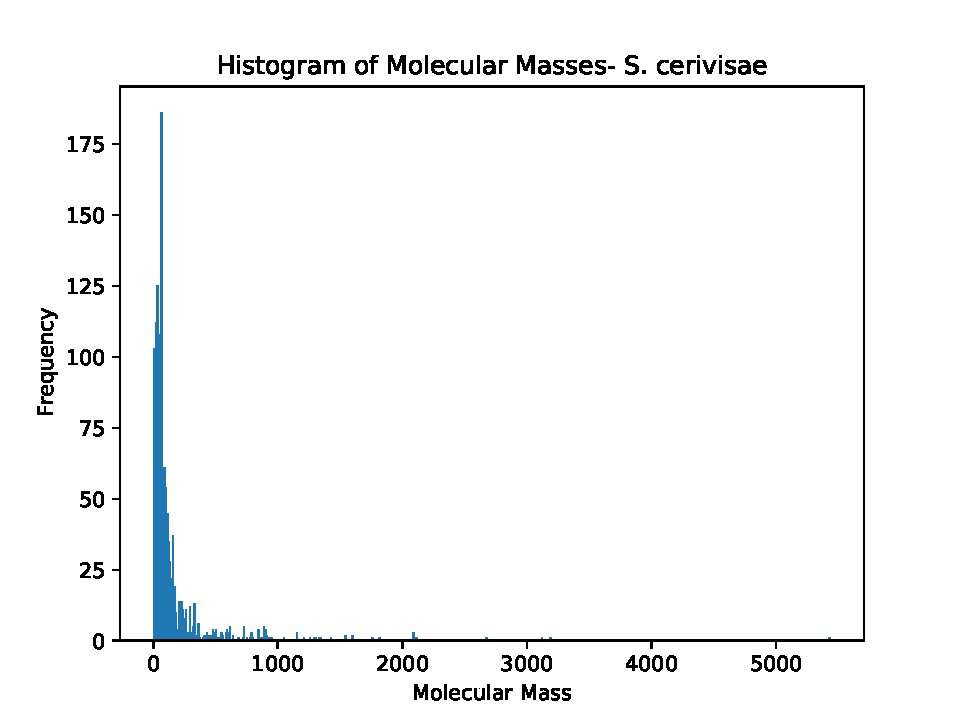
\includepdf[pages=-]{scerevisiae_mass.pdf}

\setlength{\voffset}{-2.54cm}
\setlength{\hoffset}{-2.54cm}
\subsection{Humans}
Mean of sequence length: $630.7416856492027$ \newline
Standard deviation of sequence length: $1263.078244813831$ \newline
Mean of molecular mass: $74.20564692482915$ \newline
Standard deviation of molecular mass: \newline $181.92998156053864$
\setlength{\voffset}{0cm}
\setlength{\hoffset}{0cm}

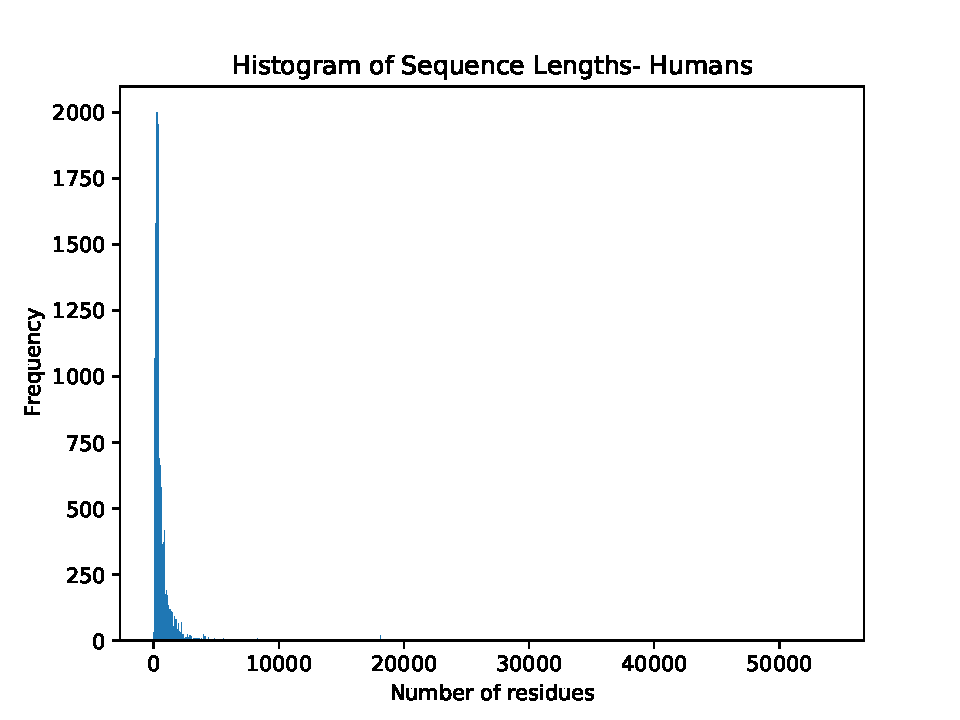
\includepdf[pages=-]{human_length.pdf}

\setlength{\voffset}{-2.54cm}
\setlength{\hoffset}{-2.54cm}
\setlength{\voffset}{0cm}
\setlength{\hoffset}{0cm}

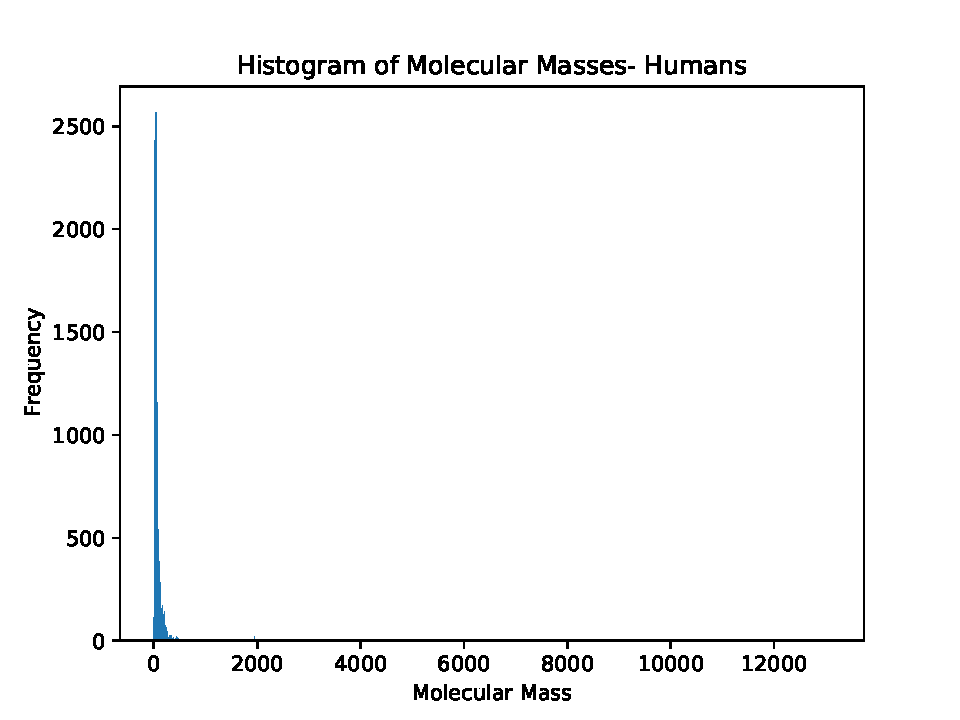
\includepdf[pages=-]{human_mass.pdf}

\setlength{\voffset}{-2.54cm}
\setlength{\hoffset}{-2.54cm}





\setlength{\voffset}{0cm}
\setlength{\hoffset}{0cm}

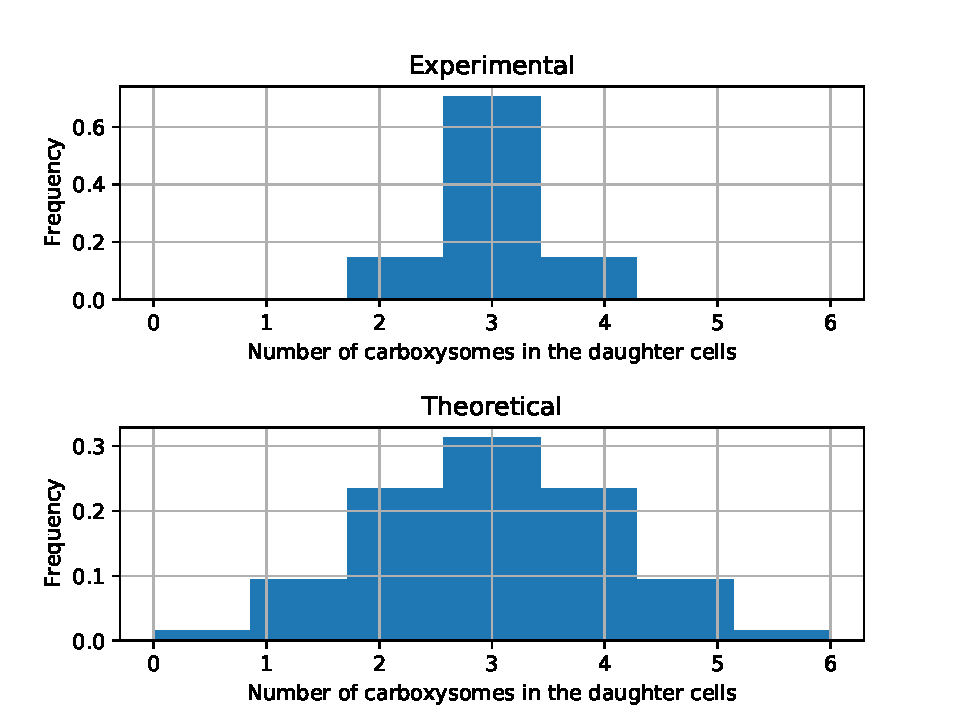
\includepdf[pages=-]{q4.pdf}

\setlength{\voffset}{-2.54cm}
\setlength{\hoffset}{-2.54cm}

(In the previous page is the histogram.)

\section{Problem 4}
The probability of having $0$ and $6$ is $$p^{3}q^{3}$$. 
The probability of having $1$ and $5$ is 
$$\binom{3}{1}p^{4}q^{2}+\binom{3}{1}p^{2}q^{4}$$
The probability of having $2$ and $4$ in one cell is
$$\binom{3}{2}p^{5}q^{1}+\binom{3}{2}p^{1}q^{5}+\binom{3}{1}\binom{3}{1}p^{3}q^{3}$$
The probability of having $3$ in one cell is
$$p^{6}+q^{6}+\binom{3}{1}\binom{3}{2}p^{2}q^{4}+\binom{3}{2}\binom{3}{1}p^{4}q^{2}$$
By substituting $p=0.5+x$, and minimizing using the least-squares method with respect to the experimental distribution, obtained value for p is $0.936093$.
Attached, is a scatter plot showing the deviation. Given that, there are only 6 molecules, and the error is about $0.007 \pm 0.001$ (for the non-zero values), I believe it's a good model.

\setlength{\voffset}{0cm}
\setlength{\hoffset}{0cm}

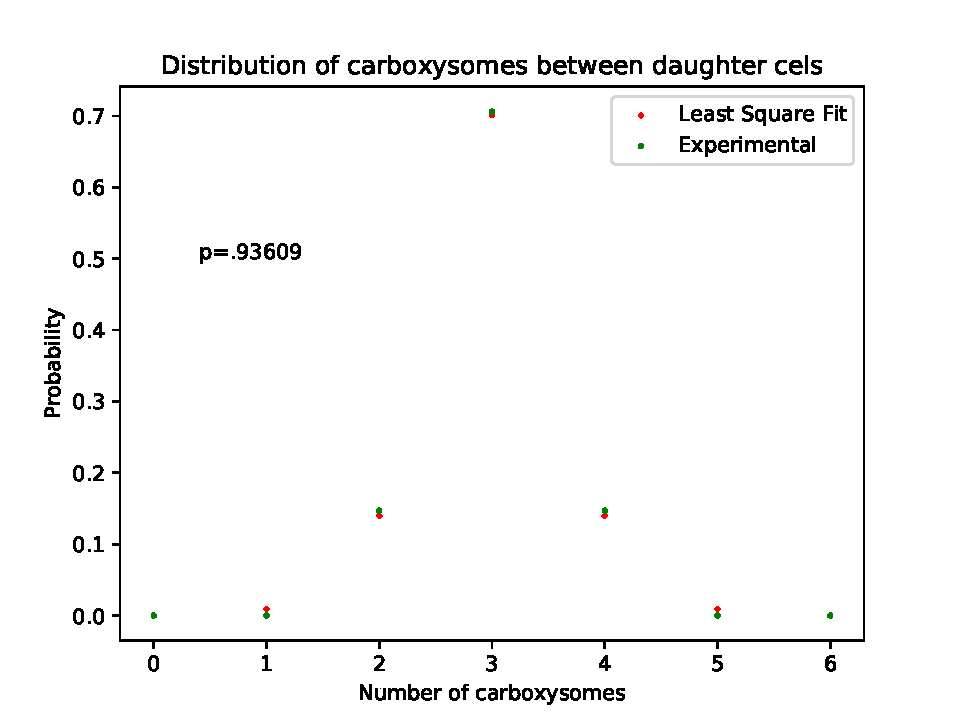
\includepdf[pages=-]{q41.pdf}

\setlength{\voffset}{-2.54cm}
\setlength{\hoffset}{-2.54cm}

\section{Problem 5}
\begin{enumerate}[label=(\alph*)]
    \item There are $4^3$ possible ways of choosing the bases to form a triplet, each with the same probability. Therefore, $$p_{s}=\frac{3}{64}$$
    % \item Let's find the probability for an unacceptable possibility. Let after $x$ bases, we get our first T base. This can be done in $3^x$ ways. We can obtain stop-codon in $3$ ways. We have $3\times N - x - 3$ bases left. These can be obtained in $4^{3N-x-3}$ ways. Therefore, the total number of ways we can get an unacceptable possibility is:
    % $$\Sigma_{x=0}^{3N-3}\left(3^{x+1}4^{3N-x-3}\right)=3\times4^{3N-3}\left(\frac{1-(\frac{3}{4})^{3N-2}}{\frac{1}{4}}\right)$$
    % Therefore, the acceptable number of possibilities are:
    % $$13\cdot4^{3N-2}+3^{3N-1}$$
    % Therefore, required probability is:
    % $$\frac{13}{16} + \frac{1}{3}\cdot \left(\frac{3}{4}\right)^{3N}$$
	\item There are 64 possible codons. Three of these are not allowed(The stop codons), to form an ORF.Therefore, the number of acceptable possibilities is $(64-3)^{N}$.\newline
	Required probability is $\left(\frac{61}{64}\right)^{N}$.
	\item Since the DNA is circular, selecting only one junction at which to start/stop reading the codon sequence suffices. \newline
	Since, there are $4$ bases, this can be done in $\binom{4}{2}= 6$ ways. 
	\item $\lfloor \frac{5\cdot 10^6}{3} \rfloor = 1666666$ and the remainder is $2$. Therefore, there are $1666666$ codons. Now, ORFs of length $600$ are desired. We can have an utmost of $ \lfloor \frac{1666666}{602} \rfloor = 2768$ ORFs (Since, at the ends of an ORF are a start and a stop codon). Each ORF(along with the start and stop codons) can be chosen in $3\cdot 61^{600}$ ways.\newline
	\item 
	\setlength{\voffset}{0cm}
\setlength{\hoffset}{0cm}

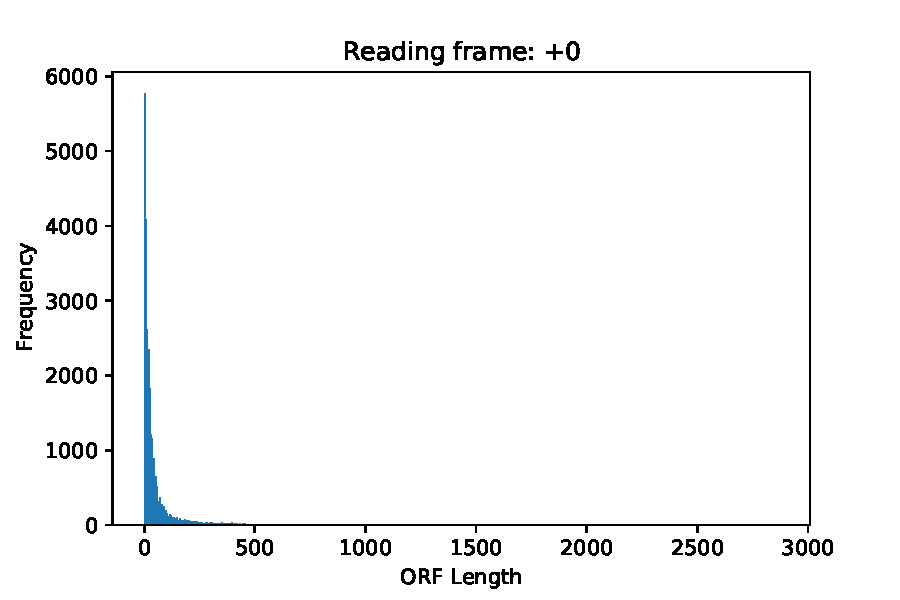
\includepdf[pages=-]{q5f0.pdf}

\setlength{\voffset}{-2.54cm}
\setlength{\hoffset}{-2.54cm}
\setlength{\voffset}{0cm}
\setlength{\hoffset}{0cm}

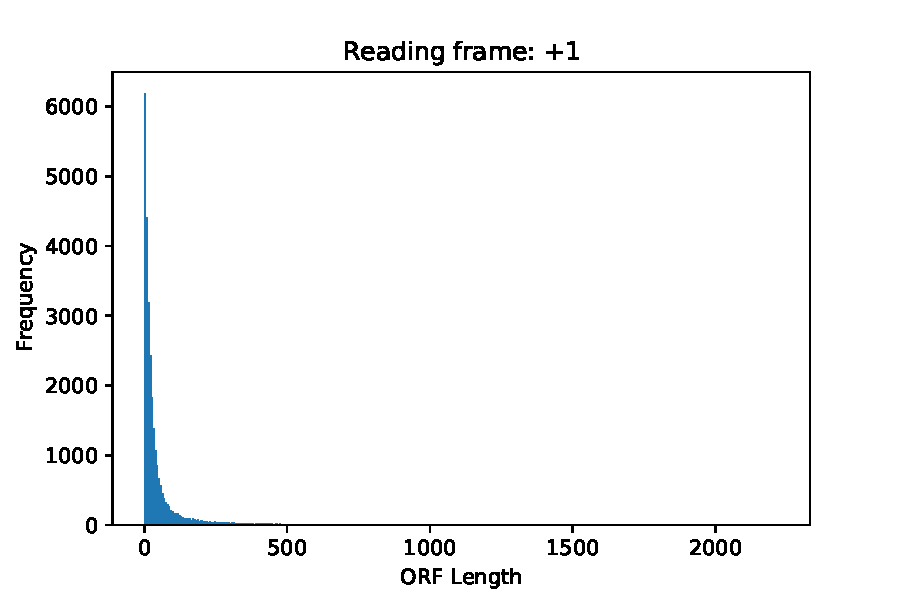
\includepdf[pages=-]{q5f1.pdf}

\setlength{\voffset}{-2.54cm}
\setlength{\hoffset}{-2.54cm}
\setlength{\voffset}{0cm}
\setlength{\hoffset}{0cm}

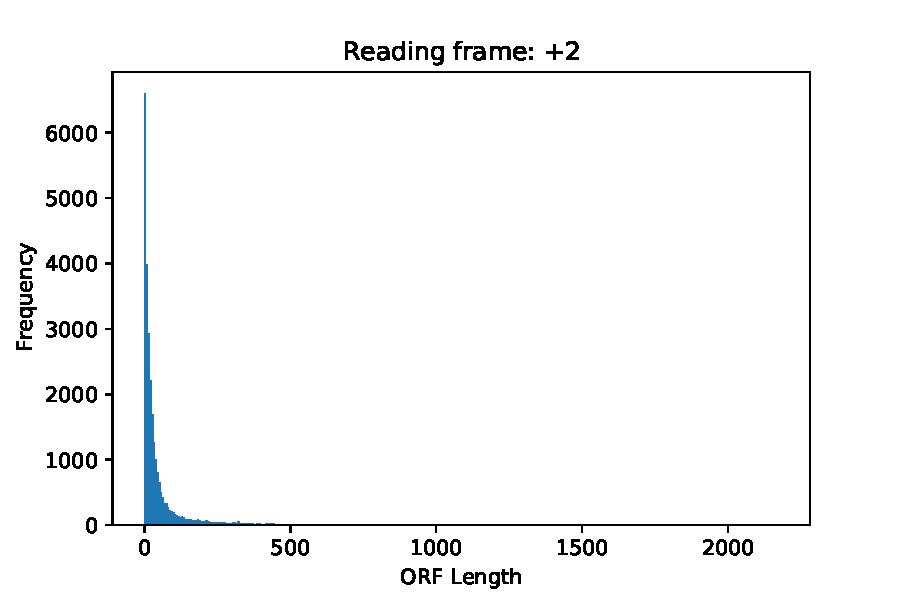
\includepdf[pages=-]{q5f2.pdf}

\setlength{\voffset}{-2.54cm}
\setlength{\hoffset}{-2.54cm}


\end{enumerate}


\end{document}